Para la realización de los tests nos concentraremos en confirmar la cota para el peor caso, el mejor caso y el comportamiento del algoritmo para casos aleatorios.

\begin{itemize}
\item El mejor caso se da cuando todos los androides están alineados en una misma fila, columna o diagonal, bajo este supuesto basta un solo kamehameha para destruirlos.
\item El peor caso se da cuando los androides están ubicados en una posición tal que cualquier semirrecta que atraviese a un par de ellos no atravesara a ninguno del resto por lo que necesitaremos una cantidad de kamehamehas igual a la mitad de los androides para destruirlos a todos. Un caso como el mencionado se da si ubicamos a los androides sobre los puntos de una parábola de una función como puede ser una cuadrática por ejemplo.
\item El otro caso se da en aquellos que no caen en ninguno de los mencionados anteriormente sino que los androides son ubicados aleatoriamente en el plano.
\end{itemize}

A continuación se muestran los resultados generados.

\begin{figure}[h!]
\begin{center}
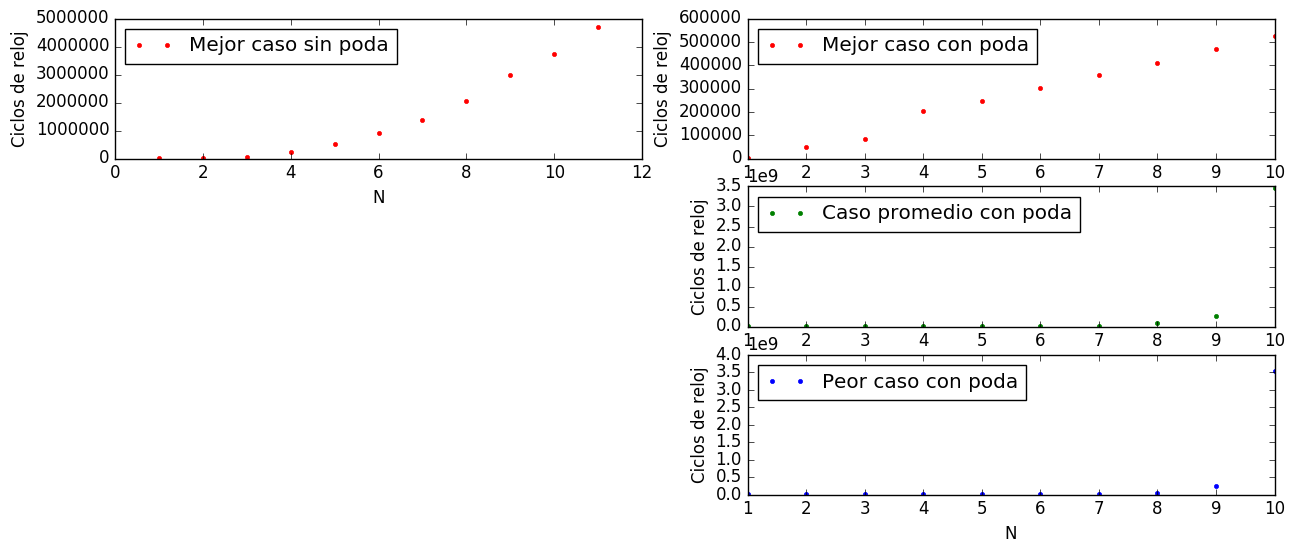
\includegraphics[width=\textwidth]{p3}
\caption{Mediciones de peor caso, mejor caso y caso promedio con y sin podas}
\end{center}
\end{figure}